\documentclass{beamer}
\usepackage{ctex}
\usepackage[export]{adjustbox}
\usepackage{listings}
\usepackage{xcolor}

\usetheme{focus}

\definecolor{codegreen}{RGB}{50 200 50}
\definecolor{codeblue}{RGB}{50 50 200}
\definecolor{codered}{RGB}{200 50 50}
\tikzset{
    global scale/.style={scale=#1,every node/.append style={scale=#1}},
    CC1/.style ={circle,minimum width = 30pt, minimum height =30pt, draw=black},
    CC2/.style ={circle,minimum width = 30pt, minimum height =30pt, draw=black, fill=blue!20},
    RA1/.style ={rectangle,minimum width = 30pt, minimum height =20pt, draw=black},
    RA2/.style ={rectangle,minimum width = 1cm, minimum height = 1cm, draw=black}
}

\title{算法分析与设计II}
\subtitle{2022-2023-2}
\date{Last Modified: 2023.1.16}
\institute{\vspace{2em} 数学与计算机学院 \\ 数据科学与大数据技术}
\titlegraphic{\vspace{5em} 
\includegraphics[scale=0.3]{fig/jlnu.pdf}}

\lstset{
    columns=flexible,       
    numbers=left,  
    numberstyle=\footnotesize\color{darkgray},  
    frame=shadowbox, 
    rulesepcolor= \color{gray}, 
    keywordstyle=\color{codeblue},         
    commentstyle=\color{codegreen},  
    stringstyle=\color{codered}, 
    showstringspaces=false,  
    xleftmargin=3em,
    xrightmargin=1em,              
    language=c++                           
}

\tikzset{
    CC1/.style ={
    circle,
    minimum width = 30pt, 
    minimum height =30pt, 
    draw=black
    }
}

\begin{document}
\frame{\titlepage}
\section{3. 基础数据结构}
\begin{frame}{3.1 堆栈}
    \begin{block}{堆栈}
        \textcolor{blue}{堆栈}(stack)是基础的数据结构,是一种\textcolor{blue}{抽象数据类型}(ADT, Abstract Data Type),其特点是后进先出(LIFO, Last In First Out)
    \end{block}
    \vfill
    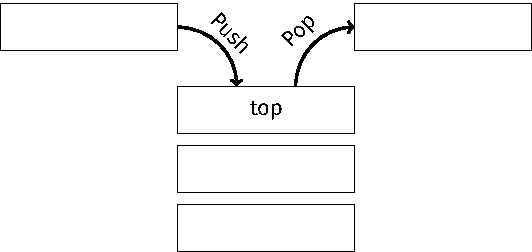
\includegraphics[center]{fig/3-1.pdf}
\end{frame}
\begin{frame}{堆栈}
    \begin{itemize}
        \item 在C++ STL中提供了专门的stack\footnote{\url{https://cplusplus.com/reference/stack/stack/}}实现堆栈的基本功能
        \vfill
        \item 手动实现栈的操作也很容易,如果空间允许,可以使用数组,预先为堆栈分配足够的空间;如果空间紧张,也可以使用链表,动态的改变堆栈的空间
        \vfill
        \item 函数的调用和返回,在计算机系统中就是通过堆栈来实现的,系统堆栈空间并不是无限的,所以限制了函数调用的层次和规模,递归算法是函数的反复调用,所以更需要注意
    \end{itemize}
\end{frame}
\vspace*{4ex}
\begin{itemize}
    \item[] \Large{堆栈基本操作}
\end{itemize}
\begin{lstlisting}
    // 将元素x加入堆栈S,S.top为栈顶位置
    // 元素入栈,栈顶位置加1
    PUSH(S,x) 
        S.top = S.top + 1 
        S[S.top] = x

    // 栈顶元素出栈,栈顶位置减1,返回栈顶元素的值
    POP(S) 
        if S.top>0
            S.top = S.top - 1
        return S[S.top + 1]
\end{lstlisting}
\begin{frame}{1363 -- Rails (poj.org)}
    \begin{itemize}
        \item 如图的车站,可以通过操作将A序列转变成B序列。现在A为1到n的顺序序列,问给出一个序列B,能否通过A生成
    \end{itemize}
    \vfill
    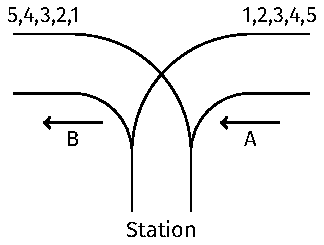
\includegraphics[center]{fig/3-2.pdf}
\end{frame}
\begin{frame}{3.2 队列}
    \begin{block}{队列}
        \textcolor{blue}{队列}(queue)也是一种抽象数据类型,其特点是先进先出(FIFO, First-In-First-Out) \\ 通常情况下,只允许在队列后端(rear)入队列(Enqueue),在队列前端(front)出队列(Dequeue)
    \end{block}
    \vfill
    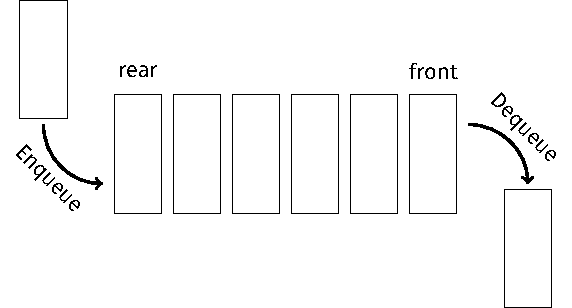
\includegraphics[scale=.8,center]{fig/3-3.pdf}
\end{frame}
\begin{frame}{队列}
    \begin{itemize}
        \item 在C++ STL中提供了专门的queue\footnote{\url{https://cplusplus.com/reference/queue/}}实现队列的基本功能
        \item 在队列的操作的过程中,每次进行1个元素的入队或者出队,不适合元素数量过多,反复进行操作
        \item 在计算机系统中,缓冲区管理就是采用队列实现,当队列空间满而没有有效检查时,会出现\textcolor{red}{缓冲区溢出}(Buffer overflow),利用系统中的缓冲区溢出是黑客攻击系统的常用手段
        \item 队列通常采用链表或者数组来实现,使用数组的时候会出现\textcolor{red}{“伪溢出”}的现象,就是数组进行一定量的入队出队操作之后,队列头还有空间,而队列尾已满而无法入队,为了解决这个问题,常常采用循环队列的方式
        \item 数组实现队列时,队列空间不方便扩展,可以采用\textcolor{blue}{链表}
    \end{itemize}
\end{frame}    
\vspace*{6ex}
\begin{itemize}
    \item[] \Large{队列基本操作}
\end{itemize}
\begin{lstlisting}
    // 将元素x加入队列Q,队列尾位置加1
    Enqueue(Q,x)
        Q[Q.rear] = x
        Q.rear = Q.rear + 1
        
    // 出队列,返回队列头元素,队列头位置加1
    Dequeue(Q)
        x = Q[Q.front]
        Q.front = Q.front + 1
        return x
\end{lstlisting}
\begin{frame}{2823 -- Sliding Window (poj.org)}
    \begin{itemize}
        \item An array of size $n\leqslant10^6$ is given to you. There is a sliding window of size $k$ which is moving from the very left of the array to the very right. You can only see the $k$ numbers in the window. Each time the sliding window moves rightwards by one position. 
    \end{itemize}
    \begin{exampleblock}{Example:The array is [1 3 -1 -3 5 3 6 7], and $k$ is 3}
    \begin{table}
    \begin{tabular}{ccc}
        Window position & Minimum value & Maximum value\\
        \hline
        [1 3 -1] -3 5 3 6 7 & -1 & 3 \\
        1 [3 -1 -3] 5 3 6 7	& -3 & 3 \\
        1 3 [-1 -3 5] 3 6 7	& -3 & 5 \\ 
        1 3 -1 [-3 5 3] 6 7	& -3 & 5 \\
        1 3 -1 -3 [5 3 6] 7	& 3 & 6 \\
        1 3 -1 -3 5 [3 6 7]	& 3 & 7 \\
        \hline
    \end{tabular}
    \end{table}
    \end{exampleblock}
\end{frame}
\begin{frame}{3.3 堆}
    \begin{block}{堆}
        \textcolor{blue}{堆}(heap)是一种特别的完全二叉树,如果完全二叉树中每个节点的值都小于等于其子节点的值,称为\textcolor{blue}{最小堆}(min heap); 反之,如果每个节点的值都大于等于其子节点的值,称为\textcolor{blue}{最大堆}(max heap)
    \end{block}
    \begin{itemize}
        \item 在C++ STL中的优先队列priority\_queue\footnote{\url{https://cplusplus.com/reference/queue/priority_queue/}}就是堆的实现,对于堆的应用可以直接使用优先队列
        \item 使用堆实现的\textcolor{blue}{堆排序}(Heapsort) ,平均时间复杂度为$O(nlogn)$
        \item 优先队列常用于计算机操作系统中的任务调度,例如基于优先级的进程调度
        \item 字符串中求最优无前缀码即哈夫曼编码,使用最小堆来实现
        \item 图论中,使用优先队列解决基于贪心思想的最小生成树等问题
    \end{itemize}
\end{frame} 
\begin{frame}{3253 -- Fence Repair (poj.org)}
    \begin{itemize}
        \item 将一个长木板进行n-1次切割,切成n个小木板,切木板的花费等于木板的长度。给出最后切割后的长度,求费用最小的切割方案
        \begin{exampleblock}{Example}
            \begin{itemize}
                \item 将21切割成8,5,8,可以先切成13和8,总费用21+13=34
                \item 如果先切成16和5,则总费用21+16=37,超过34
            \end{itemize}
        \end{exampleblock}
        \item 分析
        \begin{itemize}
            \item 假定最后切割完的所有木板在一个集合里,每次从集合中选出两个最短的,它们的和为一次切割费用,将它们合并后放回集合,重复以上操作,最后累计切割费用即可
            \item 题目的主要操作是从集合中每次取出最小的两个值,每次都重新排序的话算法复杂度会提高,而采用堆能很好的解决这个问题
        \end{itemize}
    \end{itemize}
\end{frame}
\end{document}